\graphicspath{{./images/}}

\chapter{Laufzeitsicht}

\section{Ebene 1} \textcolor{red}{TODO Titel anpassen}

\subsection{Registrierung}

Die Registrierungssequenz ist ein mehrstufiger Prozess. Hat der neu Händler ein Produkt ausgewählt und seine Kontaktdaten, Mobile-Nummer und Emailadresse, eingegeben, werden diese in der Datenbank gespeichert. Gleichzeitig wird eine Mail mit einem Registrierungslink verschickt. Sobald der Händler diese Daten erhalten hat, kann er den Prozess fortführen indem er den Link öffnet. Das Öffnen des Links löst eine SMS in Form einer MTAN aus. Mit Hilfe dieses MTANs verifiziert der Händler eine gültige Mobile-Nummer und ist damit berechtigt alle registrierungsrelevanten Daten auszufüllen und diese zu übermitteln. Die Übermittlung der Daten an die Workflow Engine erfolgt asynchron.
\begin{center}
	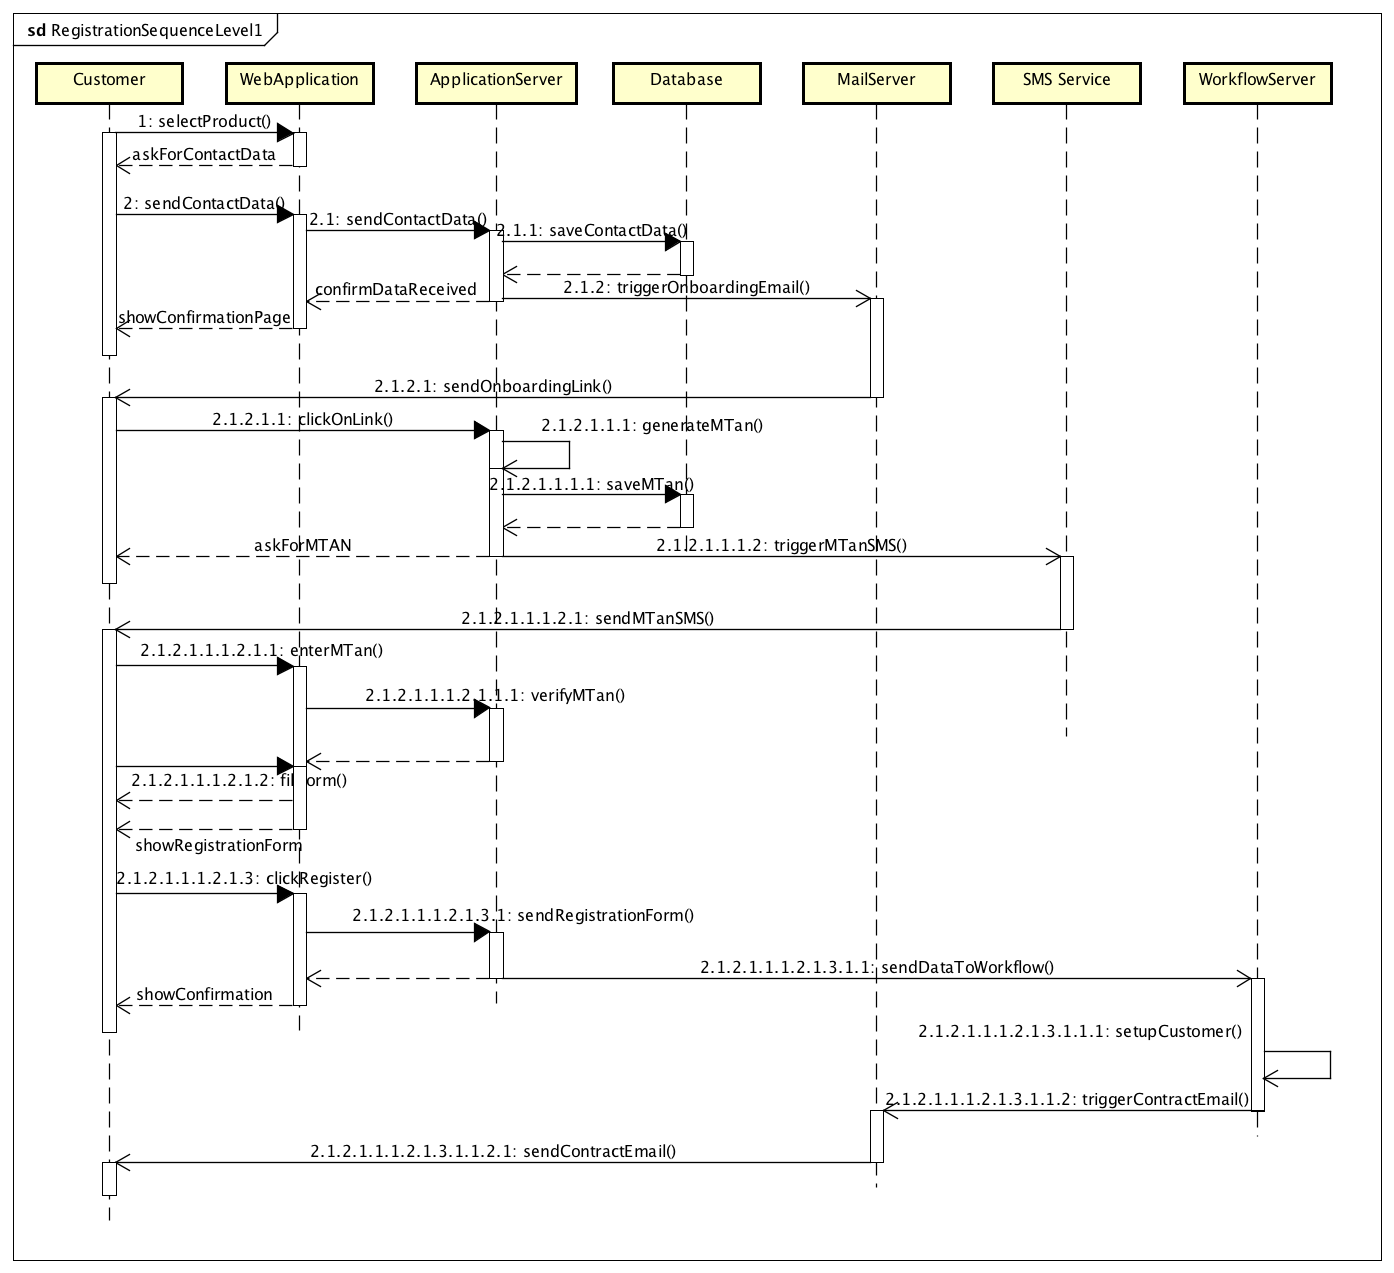
\includegraphics[scale=0.44]{RegistrationSequenceLevel1.png}
\end{center}
\newpage

\subsection{Konfigurationsänderung}

Müssen Properties der Applikation geändert werden, geschieht dies über Dateien  welche im GIT Repository eingecheckt sind. Über einen Webhook auf dem GIT Server wir über den Config Server eine Nachricht auf die Queue gelegt, wodurch die Clients die Properties updaten können. Spring Cloud Config und Spring Cloud Bus stellen alle Funktionen bereit, weshalb nur die Konfiguration des Servers, des Clients und der Queue gemacht werden muss.
\begin{center}
	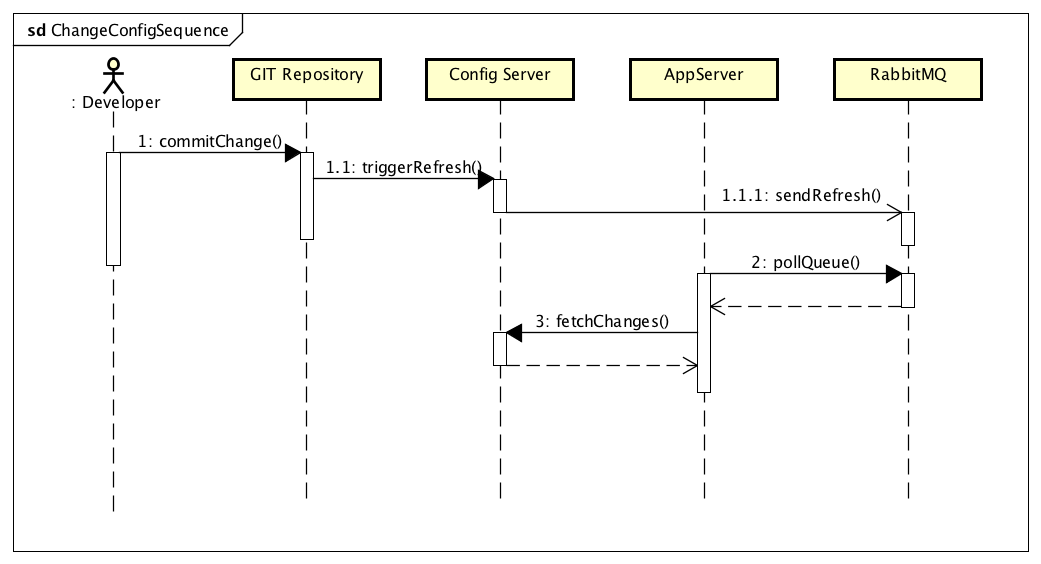
\includegraphics[scale=0.6]{ChangeConfigSequence.png}
\end{center}
\newpage
\section{Ebene 2}

Damit der Prozess der Registrierung klarer wird ist in der folgenden Abbildung der Ablauf detaillierter mit den in Kapitel \ref{reg-service} beschriebenen Komponenten dargestellt. Der SchedulerService prüft die Datenbank regelmässig und asynchron zu den Abläufen welcher der RegistrierungsService ausführt. Dadurch wird verhindert, dass der Benutzer im Fall eines Problems mit der Kommunikation zur BPM Workflow Engine etwas merkt.
\subsection{Registrierung}
\begin{center}
	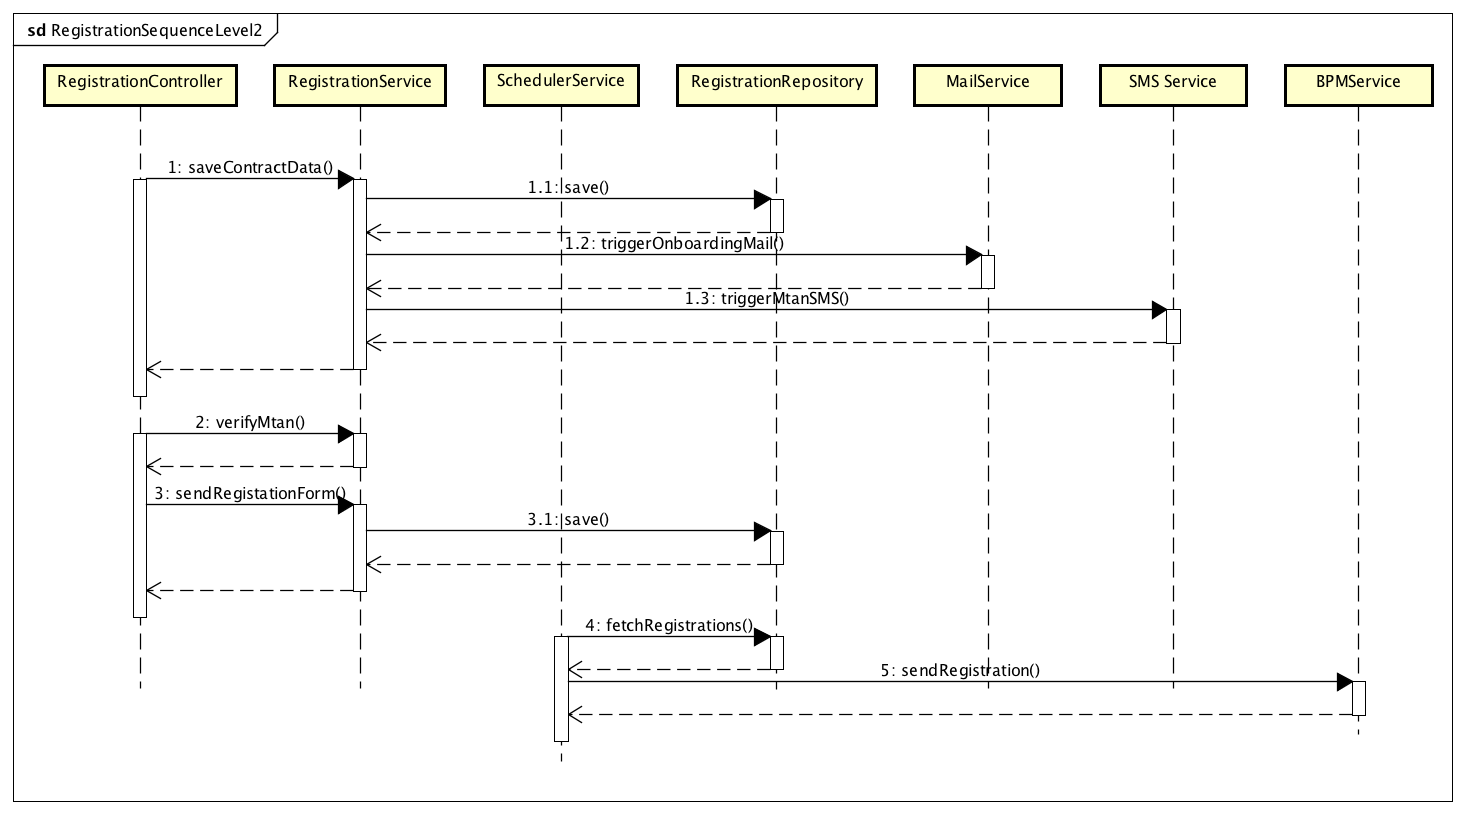
\includegraphics[scale=0.42]{RegistrationSequenceLevel2.png}
\end{center}



